\contributor{
% Add all authors
Firstname Lastname, Firstname Lastname, etc.
}
\contribution{
% Add full title
Title. Subtitle.
}
\shortcontributor{
% short version of authors for running header
Lastname et al.
}
\shortcontribution{
% short version of title for running header
Title
}

\begin{paper}
\renewcommand*{\pagemark}{}

\begin{abstract}
\lipsum[1]
\end{abstract}
%\begin{motto}
% add a motto if you need one
%\end{motto}

% YOUR PAPER STARTS HERE

% remove asterisk (*) if you want to number your sections
\section*{Introduction} 
\lipsum[2]
\lipsum[3]

% remove asterisk (*) if you want to number your sections
\section*{Headings: first level}
% use \labels for inter-document references
\label{sec:Headings} 
\lipsum[4]

% remove asterisk (*) if you want to number your sections
\subsection*{Headings: second level}
By adding the previous label, you can now refer back to Section \ref{sec:Headings} and even dynamically say that this section starts on page \pageref{sec:Headings}.

% remove asterisk (*) if you want to number your sections
\subsubsection*{Headings: third level}
For your information, here is how you add footnotes.\footnote{Sample of the first footnote.}

\paragraph{Paragraph}
\lipsum[7]

% remove asterisk (*) if you want to number your sections
\section*{Examples figures and tables}
\label{sec:Others}
\lipsum[8] 

You can use ``in-text \textbf{citations}''\citep[see][5]{wiki:xx2}; see also \cite{wiki:xx2}. Or you can use block quotes:

\begin{quote}
LaTeX [...] is a document markup language and document preparation system for the TeX typesetting program. Within the typesetting system, its name is styled as \LaTeX. The term LaTeX refers only to the language in which documents are written, not to the editor used to write those documents. In order to create a document in LaTeX, a .tex file must be created using some form of text editor. While most text editors can be used to create a LaTeX document, a number of editors have been created specifically for working with LaTeX.

\citep{wiki:xx2}
\end{quote}

\subsection*{Figures}
See Figure \ref{fig:demographic}: 


\begin{figure}[H]
  \centering
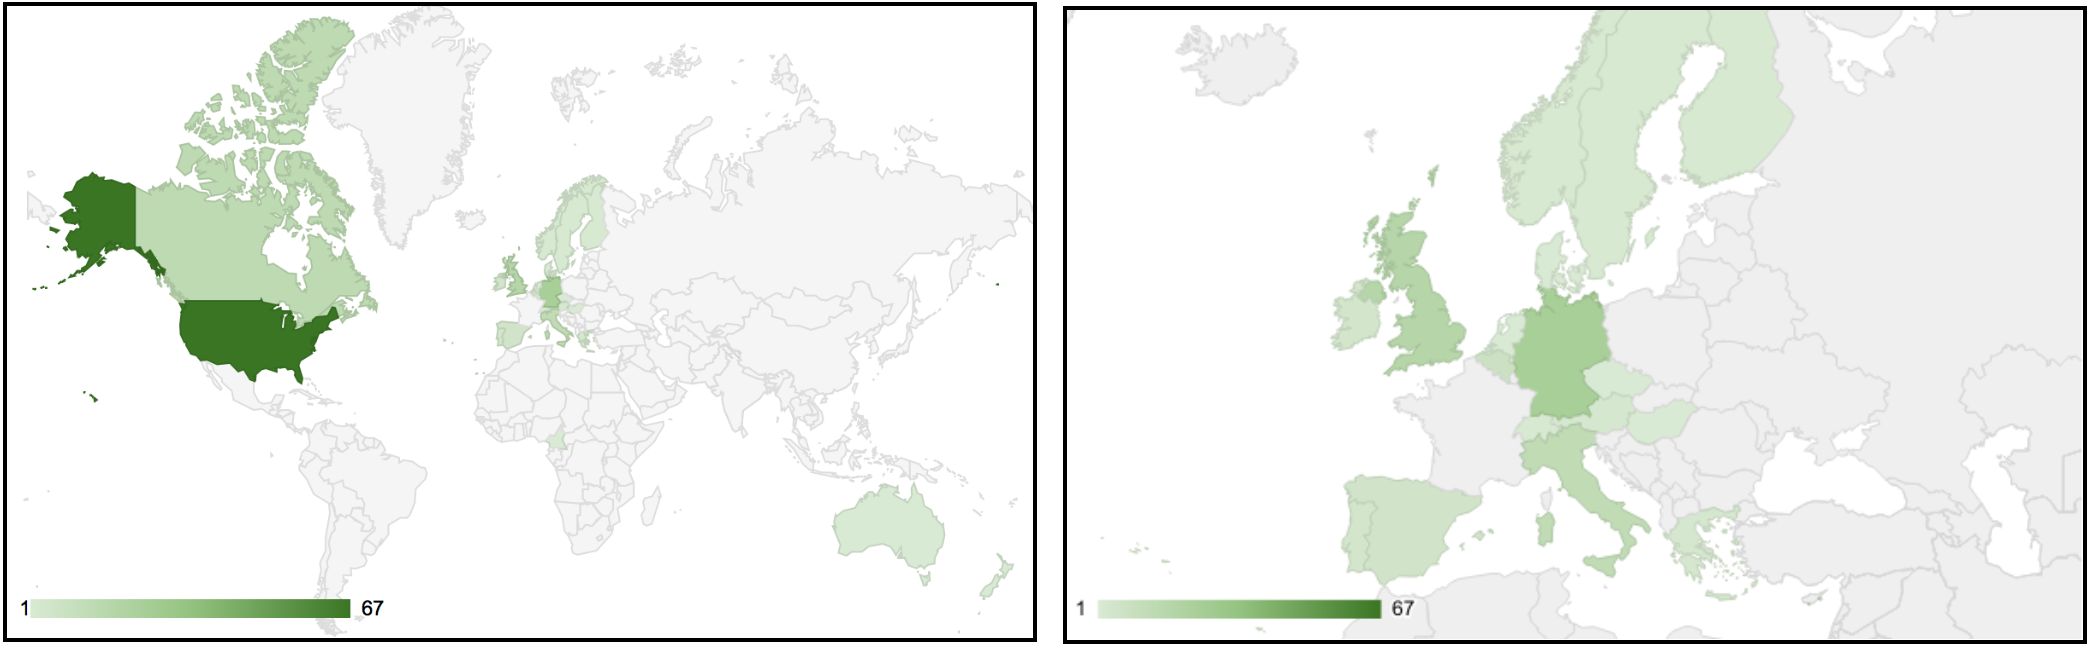
\includegraphics[width=\textwidth]{media/martinez1.png}  \caption{Sample figure caption.}
  \label{fig:demographic}
\end{figure}

\subsection*{Tables}
\lipsum[12]
See  Table~\ref{tab:table}.

\begin{table}[H]
 \caption{Sample table title}
  \centering
  \begin{tabular}{lll}
    \toprule
    \multicolumn{2}{c}{Part}                   \\
    \cmidrule(r){1-2}
    Name     & Description     & Size ($\mu$m) \\
    \midrule
    Dendrite & Input terminal  & $\sim$100     \\
    Axon     & Output terminal & $\sim$10      \\
    Soma     & Cell body       & up to $10^6$  \\
    \bottomrule
  \end{tabular}
  \label{tab:Table}
\end{table}


\bibliography{essays/empty-template-references}  


\end{paper}